\section{Methods}
\label{sec:methods}

% \begin{figure*}
% % \begin{minipage}{\textwidth}
%   \centering
%   \begin{minipage}{.45\textwidth}
%      \centering
%         % \begin{algorithm}
%         % \caption{Extending episodic learning to multiple tasks in the training corpus. SAMPLE$(S,K)$ denotes selecting $K$ samples uniformly at random from set $S$ with replacement.}
%         % \label{algo:ProtoNet}
%         \hspace*{\algorithmicindent} \textbf{Input:} T: set of tasks, N: number of episodes
%         \begin{algorithmic}[1]
%         \For{i $\in \{1...N\}$}
%             \State $t \gets $SAMPLE$(T,1)$. \Comment{Sample a task}
%             \For{c in $\{1...C\}$}
%                 \State $D_{t,c} \gets$ Embeddings $\in$ class $c$ in task $t$
%                 \State $S_{t,c} \gets $SAMPLE$(D_{t,c},k)$ \Comment{k supports}
%                 \State $Q_{t,c} \gets $SAMPLE$(D_{t,c},q)$ \Comment{q queries}
%             \EndFor
%             \State Perform Episodic Training: Equations (\ref{eqn:proto_basic}-\ref{eqn:proto_backprop})
%         \EndFor
%         \end{algorithmic}
%         % \end{algorithm}
%   \end{minipage}
%   \begin{minipage}{.45\textwidth}
%      \centering
%         % \begin{algorithm}
%         % \caption{Extending episodic learning to multiple tasks in the training corpus. SAMPLE$(S,K)$ denotes selecting $K$ samples uniformly at random from set $S$ with replacement.}
%         % \label{algo:ProtoNet}
%         \hspace*{\algorithmicindent} \textbf{Input:} T: set of tasks, N: number of episodes
%         \begin{algorithmic}[1]
%         \For{i $\in \{1...N\}$}
%             \State $t \gets $SAMPLE$(T,1)$. \Comment{Sample a task}
%             \For{c in $\{1...C\}$}
%                 \State $D_{t,c} \gets$ Embeddings $\in$ class $c$ in task $t$
%                 \State $S_{t,c} \gets $SAMPLE$(D_{t,c},k)$ \Comment{k supports}
%                 \State $Q_{t,c} \gets $SAMPLE$(D_{t,c},q)$ \Comment{q queries}
%             \EndFor
%             \State Perform Episodic Training: Equations (\ref{eqn:proto_basic}-\ref{eqn:proto_backprop})
%         \EndFor
%         \end{algorithmic}
%         % \end{algorithm}
%   \end{minipage}
%   \caption{figure}{Two algorithms side by side}
%   \label{fig:twoalg}
% % \end{minipage}
% \end{figure*}

In this section, we introduce the meta-learning setup for neural embedding training followed by description of two metric-learning approaches adopted in this work: prototypical networks and relation networks. Following which, we outline their use in our tasks: speaker diarization and speaker verification, including a description of the choice of clustering algorithm.

Consider a training corpus where $C$ denotes the set of unique speakers, and where each speaker has multiple utterances available. Typically, $|C|$ is a large integer
($\mathcal{O}(10^3)$).  
Here, an utterance might be in the form of raw waveform or frame-level features such as MFCCs or Mel spectrogram. 
%During conventional classification, a minibatch is randomly sampled from the training corpus wherein both the speakers and number of samples per speaker are simultaenously sampled. The final layer in a DNN is fixed-dimensional, i.e $N$. 
Under the meta-learning setup, each episode (a training step; equivalent to a minibatch) consists of two stages of sampling: classes and utterances conditioned on classes. 
First, a subset of classes $L$ (speakers) is sampled from $C$ within an episode, with the number of speakers per episode $|L|$ typically held constant during the training process. 
Next, two disjoint sets from each speaker in $L$ are sampled without replacement from the set of all utterances belonging to that speaker: supports $S$ and queries $Q$. 
Within an episode, supports and queries are used for model training and loss computation, respectively, similar to train and test sets in supervised training. This process continues across a large number of episodes with speakers and utterances sampled as explained above.
Following terminology from Section \ref{sec:intro}, an episode is equivalent to a \textit{task}, wherein the model learns to classify speakers from that task. Hence, meta-learning optimizes across tasks, treating each task as a training example. The optimization process is given as:
\begin{equation}
    \theta = \argmax_{\theta} \displaystyle \mathop{\mathbb{E}}_{L} [ \mathop{\mathbb{E}}_{S, Q} [ \mathop{\mathbb{E}}_{(\mathbf{x},y) \in Q} [ \log p_\theta (y|\mathbf{x},S)] ]]
\end{equation}
% \begin{equation}
%     \theta = \argmax_{\theta} \displaystyle \mathop{\mathbb{E}}_{L \sim C} [ \mathop{\mathbb{E}}_{\substack{S \sim L\\ Q \sim L}} [ \mathop{\mathbb{E}}_{(x,y) \in Q} \log p_\theta (y|x,S) ]]
% \end{equation}
Here, $\theta$ denotes trainable parameters of the neural network, $(\mathbf{x},y)$ represents an utterance and its corresponding speaker label. In contrast to conventional supervised learning:
\begin{equation}
    \theta = \argmax_{\theta} \displaystyle \mathop{\mathbb{E}}_{B} [  \mathop{\mathbb{E}}_{(\mathbf{x},y) \in B}[\log p_\theta (y|\mathbf{x})]  ]
\end{equation}
where $B$ denotes a minibatch. Meta-learning approaches are broadly categorized based on the characterization of $p_\theta (y|x)$: model-based \cite{santoro2016meta}, metric-based \cite{vinyals2016matching} and optimization-based meta-learning \cite{finn_maml2017}. 
Of interest in this work are metric-based approaches where $p_\theta (y|x)$ is a potentially learnable kernel function between utterances from $S$ and $Q$. The reasoning is as follows: speaker embeddings trained for classification are bottleneck representations, and the latter is directly optimized using task performance in metric-learning approaches. We now describe the two metric-learning approaches used in this work: prototypical networks and relation networks.

\subsection{Prototypical Networks}

Protonets learn a non-linear transformation where each class is represented by a single point in the embedding space, namely the centroid (prototype) of training utterances from that class. During inference a test sample is assigned to the class of nearest centroid, similar to the nearest class mean method \cite{mensink2013}. 

At training time, consider an episode $t$, the support set ($S_t$) and the query set ($Q_t$) sampled as explained above. Supports are used for prototype computation while queries are used for estimating class posteriors and loss value. 
%Protonets learn the mapping $f_{\theta} : \mathbb{R}^M \rightarrow \mathbb{R}^P$ where the prototype of each class is computed as follows:
The prototype ($\mathbf{v}_c$) for each class is computed as follows:
\begin{equation}
\label{eqn:proto_basic}
    \mathbf{v}_{c} = \frac{1}{|S_{t,c}|} \sum_{(\mathbf{x_{i}},y_{i})\in S_{t,c}} f_{\theta}(\mathbf{x}_i)
\end{equation}
$f_{\theta} : \mathbb{R}^M \rightarrow \mathbb{R}^P$ represents the parameters of the protonet. $\mathbf{x_i}$ represents an $M$-dimensional utterance representation extracted using a DNN.
$S_{t,c}$ is the set of all utterances in $S_t$ belonging to class $c$. For every test utterance $\mathbf{x_j} \in Q_t$, the posterior probability is computed by applying softmax activation over the negative distances with prototypes:
\begin{equation}
\label{sofmax-eq2}
    p_\theta(y_j=c\,| \mathbf{x}_j, S_t)=\frac{\exp \left(-d\left(f_{\theta}(\mathbf{x}_j), \mathbf{v}_c\right)\right)}{\sum_{c^{\prime} \in L} \exp \left(-d\left(f_{\theta}(\mathbf{x}_j), \mathbf{v}_{c^{\prime}}\right)\right)}
\end{equation}
$d$ represents the distance function. 
Squared Euclidean distance was proposed in the original formulation \cite{snell2017prototypical} due to its interpretability as 
a Bregman divergence \cite{banerjee2005} as well as supporting empirical results. For the above reasons, we adopt squared Euclidean as a metric in this work.
The negative log-posterior is treated as the episodic loss function and minimized using gradient descent:
\begin{equation}
\label{eqn:proto_backprop}
 \text{Loss} = - \frac{1}{|Q_t|} \sum_{(\mathbf{x}_j,y_{j})\epsilon Q_t } \log(p_\theta(y_j \mid \mathbf{x}_j, S_t)) 
\end{equation}

\subsection{Relation Networks}

Relation networks compare supports and queries by learning the kernel function simultaneously with the embedding space\cite{sung2018learning}. In contrast with protonets which use squared Euclidean distance, relation networks learn a more complex inductive bias by parameterizing the comparison metric using a neural network. 
Hence, relation networks attempt to jointly learn the embedding and metric over an ensemble of tasks that are generalized to an unseen task. Specifically, there exist two modules: an encoder network that maps utterances into fixed-dimensional embeddings and a comparison network that computes a scalar relation given pairs of embeddings. Given supports $S_t$ within an episode $t$, the class representation is taken as the sum of all support embeddings:
\begin{equation}
\label{eqn:relation_encoder}
    \mathbf{v}_c = \sum_{(\mathbf{x}_i,y_{i})\epsilon S_{t,c}} f_{\theta}(\mathbf{x}_i)
\end{equation}
$f_{\theta}$ represents the encoder network. For each query embedding belonging to a class $j$, its relation score $r_{c,j}$ with training class $c$ is computed using the comparison network $g_{\phi}$ as follows:
\begin{equation}
\label{eqn:relation_relation}
    r_{c,j} = g_{\phi} ([ \mathbf{v}_c, f_{\theta} (\mathbf{x}_j) ])
\end{equation}
Here $[.,.]$ represents concatenation operation. The original formulation of relation networks \cite{sung2018learning} treated the relation score as a similarity measure, hence $r_{c,j}$ is trained with:

\begin{equation}
    r_{c,j}= 
\begin{cases}
    1, & \text{if } y_j = c\\
    0, & \text{otherwise}
\end{cases}
\end{equation}

In the original formulation \cite{sung2018learning}, the networks $f_\theta$ and $g_\phi$ were jointly optimized using mean squared error (MSE) objective since the predicted relation network was treated similar to a linear regression model output. In this work, we replace MSE with the conventional cross-entropy objective based on empirical results. Hence the posterior probability is computed as:
\begin{equation}
\label{softmax-eq}
    p_\theta(y_j| \mathbf{x_j}, S_t)=\frac{\exp \left(  r_{c,j}   \right)}{\sum_{c^{\prime} \in L} \exp \left(    r_{c^{\prime},j}     \right)}
\end{equation}
and the loss function is computed using Eq. \ref{eqn:proto_backprop}.

\subsection{Use in Speaker Applications}

\subsubsection{Speaker Diarization}
\label{subsubsec:bSCNME}
Typically, there exist four steps in a speaker diarization system: speech activity detection, speaker segmentation, embedding extraction and speaker clustering (exceptions include recently proposed end-to-end approaches \cite{horiguchi2020endtoend,fujita2020endtoend}). In this work, we adopt the uniform segmentation strategy similar to \cite{Sell2018_dihard, garciaRomero2017} wherein the session is segmented into equal duration segments with overlap. Meta-learned embeddings are extracted from these segments followed by clustering. We use a recently proposed variant of spectral clustering \cite{park_SC2020} which uses a binarized version of affinity matrix between speaker embeddings. The binarization is expressed using a parameter ($p$) which represents the fraction of non-zero values at every row in the affinity matrix.
The clustering algorithm attempts a tradeoff between pruning excessive connections in the affinity matrix (minimizing $p$) while increasing the normalized maximum eigengap (NME; $g_p$) where the latter is expressed as a function of $p$ (Eq. (10) in \cite{park_SC2020}). The ratio ($\frac{p}{g_p}$) is then minimized to estimate the number of resulting clusters (i.e., speakers) in a session. This process is referred to as binarized spectral clustering with normalized maximum eigengap (NME-SC).

Our choice of NME-SC in this work is motivated by two reasons: (1) We do not require a separate development set to estimate a threshold parameter used in the more common agglomerative hierarchical clustering (AHC) method with average linking applied on distances estimated using probabilistic linear discriminant analysis (PLDA) \cite{Sell2018_dihard}. We choose the binarization parameter ($p$) for each session by optimizing for ($\frac{p}{g_p}$) over a pre-determined range for $p$. (2) Empirical results which demonstrate similar performance between AHC tuned on a development set and NME-SC reported in \cite{park_SC2020} and in this work. 

\subsubsection{Speaker Verification}
We use the standard protocol for speaker verification wherein a speaker embedding is extracted from the entire utterance. Subsequently, the embeddings are reduced in dimension using LDA and trial pairs are scored using a PLDA model trained on the same data used to train embeddings. Following this, target/imposter pairs are determined using a threshold on the PLDA scores.

\begin{figure*}
    \centering
    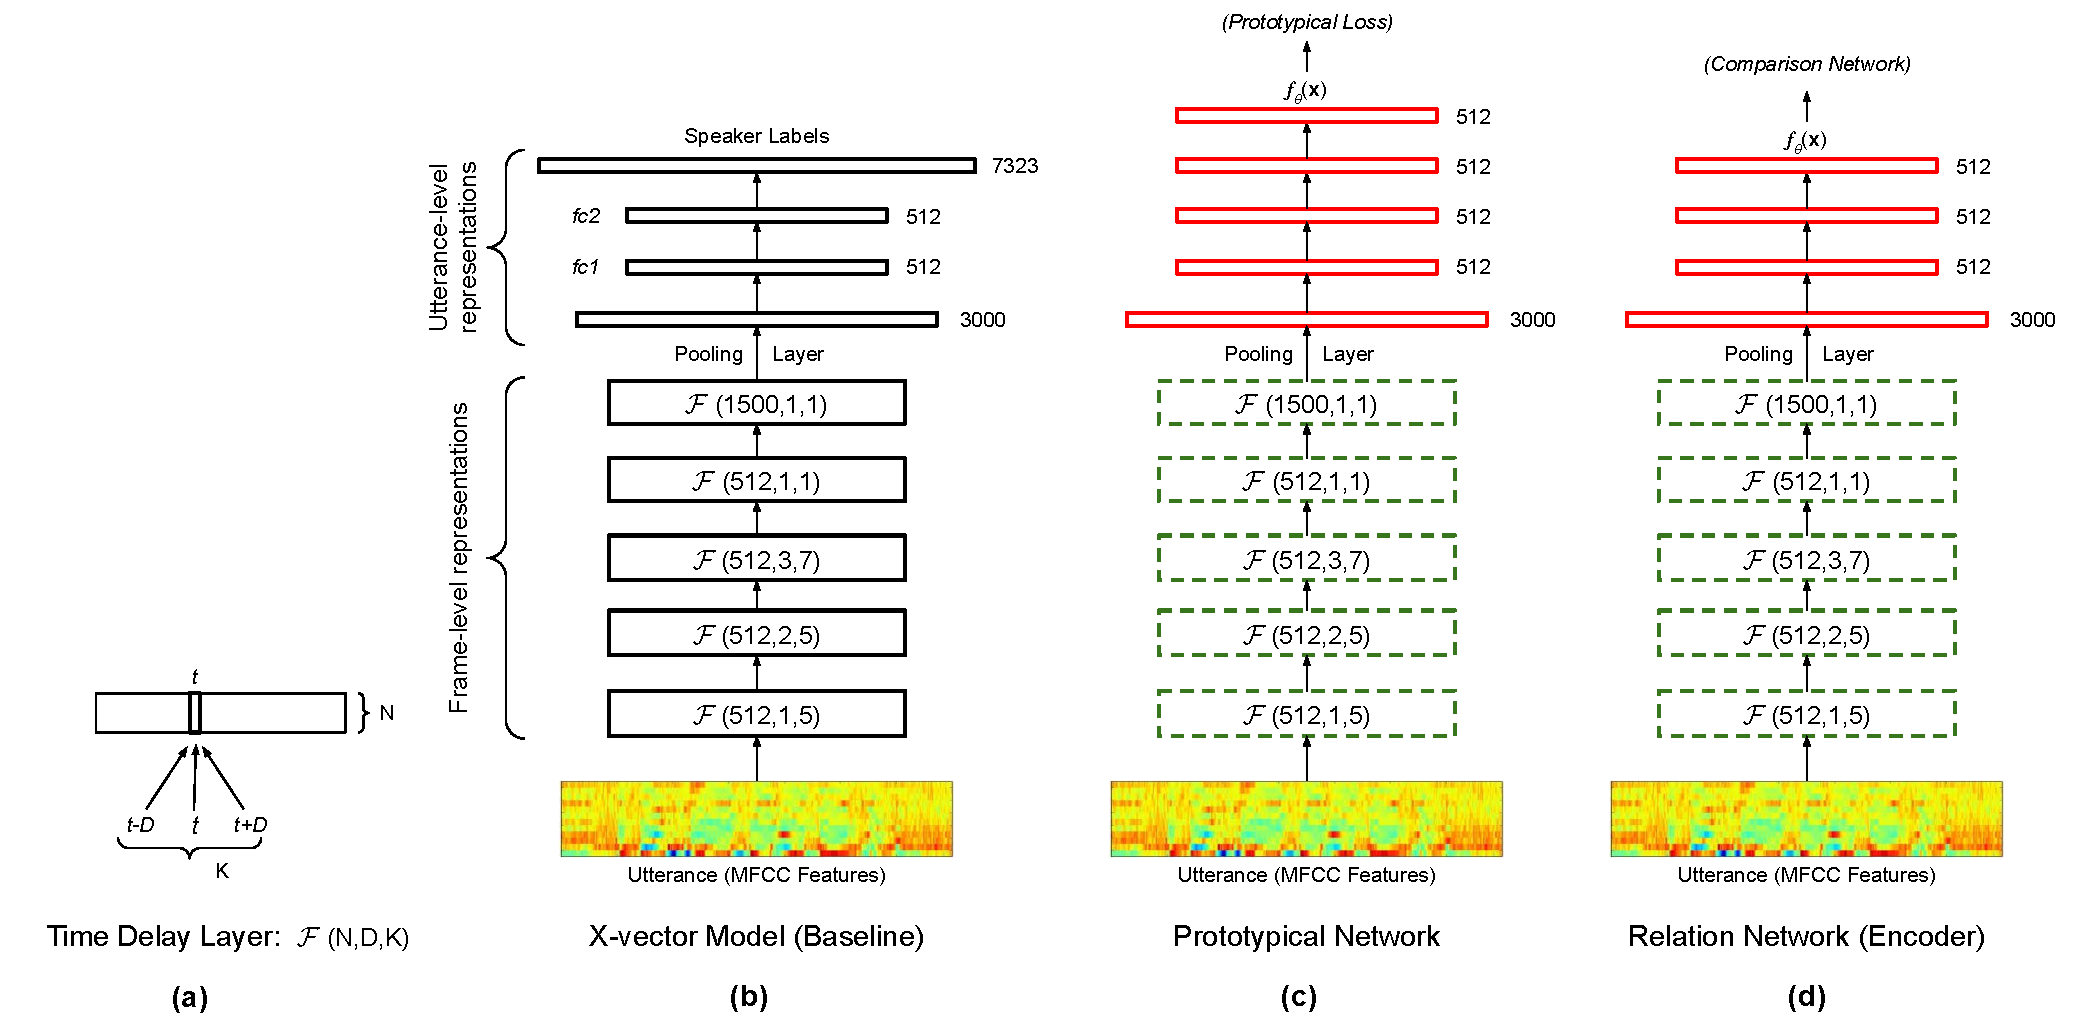
\includegraphics[width=\textwidth]{fig/meta_learning_arch.pdf}
    \caption{Overview of baseline and meta-learning architectures. \textbf{(a)} A time-delay layer $\mathcal{F}(N,D,K)$ which forms the basic component across models. At each time-step, activations from the previous layer are computed using a context width of $K$ and a dilation of $D$. $N$ represents the output embedding dimension. \textbf{(b)} Baseline x-vector model. Kaldi speaker embeddings are extracted at fc1 layer. We find that fc2 and fc1 embeddings perform better for speaker diarization and speaker verification respectively. \textbf{(c)} Prototypical network architecture. Layers marked with a dashed boundary are initialized with pre-trained x-vector models, while layers with a solid boundary are randomly initialized. The final layer output is referred to as protonet embeddings. \textbf{(d)} Relation encoder architecture. The final layer output is referred to as relation network embeddings. Relation scores are computed used these embeddings as illustrated in Fig. \ref{fig:metaLearningLoss}b) }
    \label{fig:metaLearningArch}
\end{figure*}


% Talk about the evaluation methods for each application
% % Speaker Diar
% We use DER, which is .....
% We do not use any collar, like the recent DIHARD. However, we do remove overlapping regions since neither baseline nor proposed systems take it into account
% We assume VAD is available in all our experiments 

% % SV
% We use EER, which is